\documentclass{article}

% Packages for formatting and special symbols
\usepackage{amsmath}
\usepackage{amssymb}
\usepackage{graphicx}
\usepackage{caption}
\usepackage{subcaption}
\usepackage{hyperref}
\usepackage{geometry}
\usepackage{fancyhdr}
\usepackage{setspace}
\usepackage{enumitem}
\usepackage{float}

\graphicspath{ {./graphs/} }

% Page layout
\geometry{top=1in, bottom=1in, left=1in, right=1in} % Adjust margins as needed
\pagestyle{fancy}
\fancyhf{}
\rhead{Matic Stare}
\lhead{Identifikacija relevantnih značilk za klasifikacijo alfa ritmov}
\cfoot{\thepage}
\renewcommand{\headrulewidth}{0.4pt}
\renewcommand{\footrulewidth}{0.4pt}
\renewcommand{\figurename}{Slika}
\begin{document}
% Title
\title{Identifikacija relevantnih značilk za klasifikacijo alfa ritmov}
\author{Matic Stare}
\date{\today}

\maketitle

\begin{abstract}
    V tem poročilu bomo predstavili postopek, ki smo ga uporabili pri izbiri značilk za klasifikacijo alfa ritmov iz EEG signalov. V ta namen smo napisali program, ki nam je pomagal pri izbiri značilk. Na koncu smo izbrali značilko z najvišjo vrednost kriterija $R^2$ in na njej izračunali moč signala.
\end{abstract}

% Sections
\section{Uvod}
\label{sec:introduction}

Preden začnemo s klasifikacijo EEG signalov je potrebno najprej izbrati ustrezne značilke. V ta namen smo v programskem jeziku MATLAB implementirali algoritem, ki nam pomaga pri izbiri značilk za klasifikacijo alfa ritmov iz EEG signalov, ki smo jih pridobili iz podatkovne baze EEGMMI. Ta je dostopna na povezavi \href[]{https://www.physionet.org/content/eegmmidb/1.0.0/}{Physionet}. V nadaljevanju bomo opisali postopek, ki smo ga uporabili pri njihovi izbiri.


\section{Metode}
\label{sec:methodology}

Iz podatkovne baze EEGMMI smo naključno izbrali en subjekt (številka 20). Ta vsebuje 14 različnih datotek s signali. Za branje EEG signalov, pa smo si pomagali s paketom WFDB. Ker želimo izbrati značilke za klasifikacijo alfa ritmov, smo izbrali prvo datoteko, kjer je imel subjekt odprte oči in v nadaljevanju služi kot \emph{baseline} posnetek. Potem smo izbrali še datoteke 3, 7 in 11, kjer je subjekt izvajal prvo mentalno vajo (odpiranje in zapiranje leve ali desne pesti). Z namenom, da bi bili naši podatki čim bolj reprezentativni, smo izračunali povprečje slednjih datotek in ga uporabili kot \emph{mean} posnetek. Ko smo pridobili in uredili navedene podatke, smo \emph{mean} s pomočjo Fourierjeve transformacije pretvorili v frekvenčni prostor. Nato smo ga razdelili na 10 frekvenčnih pasov in s pomočjo inverzne Fourierjeve transformacije prevedli nazaj. Potem smo vsakemu pasu s pomočjo kriterija $R^2$ izračunali koeficient z \emph{baseline} posnetkom. Dobljeno matriko smo vizualizirali s pomočjo \emph{heatmap-a}. Na njem smo izbrali polje z najvišjo vrednostjo in na signalu, ki mu pripada, in ustreznem frekvenčnem pasu izračunali moč. 



\section{Rezultati}
\label{sec:results}

Na Sliki \ref{fig:r2} so prikazane mape značilk na osnovi kriterija $R^2$. Temno modra barva predstavlja večjo korelacijo med posnetkoma, kot bela. Vidimo lahko, da je največji koeficient na 64. kanalu v 10. frekvenčnem pasu. Zato smo ta signal uporabili naprej in na njem izračunali njegovo moč. To smo skupaj s podatkom o časovni oznaki vizualizirali na Sliki \ref{fig:power}, kjer je prikazana moč signala 64. kanala 10. frekvenčnega pasu v odvisnosti od časa.


\begin{figure}[H]
    \begin{subfigure}{0.49\linewidth}
        \centering
        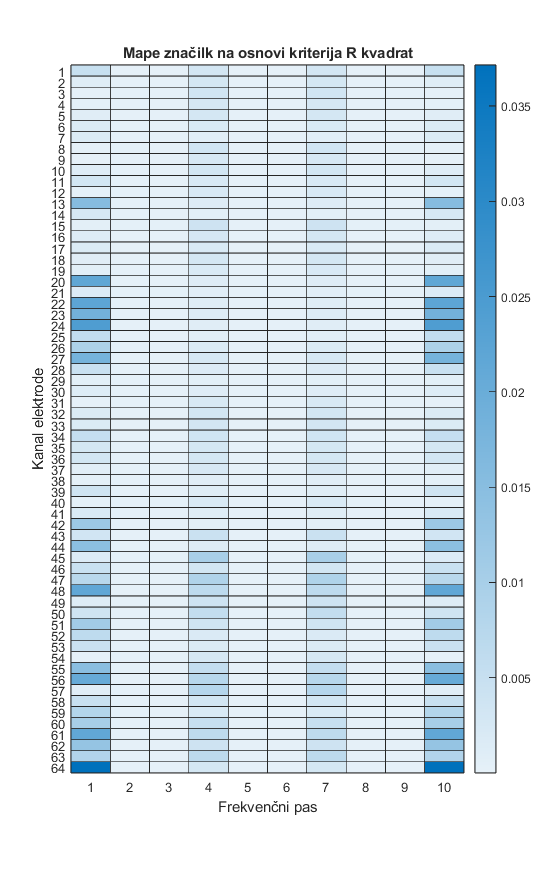
\includegraphics[width=\textwidth]{r2.png}
        \caption{Mape značilk na osnovi kriterija R kvadrat.}\label{fig:r2}
    \end{subfigure}
   \begin{subfigure}{0.49\linewidth}
        \centering
        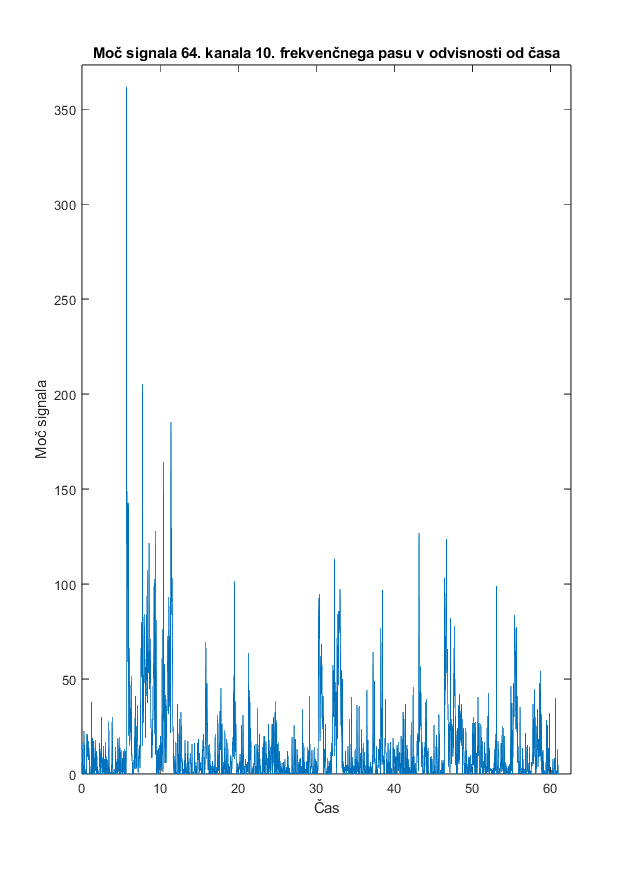
\includegraphics[width=\textwidth]{power.png}
        \caption{Moč signala 64. kanala 10. frekvenčnega pasu v odvisnosti od časa.}\label{fig:power}
    \end{subfigure}
    \caption{Grafa}\label{fig:graphs}
\end{figure}


\section{Diskusija}
\label{sec:discussion}

Iz Slike \ref{fig:r2} lahko razberemo, da so vrednosti izjemno majhne. To je posledica dejstva, da vaja, ki jo je subjekt izvajal, ne vsebuje premikanje oči. Kot možnost za nadaljnje delo bi lahko pridobili posnetke, v katerih subjekt to počne, in podobno analizo izvedli na njih.

\end{document}